\documentclass[]{beamer}

\usepackage{tikz}
\usetikzlibrary{shapes.geometric, arrows}
\tikzstyle{result} = [rectangle, rounded corners, minimum width=3cm, minimum height=0.5cm, text centered, draw=black, fill=green!30]
\tikzstyle{process} = [rectangle, minimum width=3cm, minimum height=0.5cm, text centered, draw=black, fill=orange!30]
\tikzstyle{arrow}= [thick,->,>=stealth]
\usepackage{movie15}
\usepackage{lipsum}
\usepackage{pgfpages}
\usepackage{graphicx}
\usepackage[dutch]{babel}
\graphicspath{{img/}}

\mode<handout>{%
%	\setbeameroption{show notes}
}

\usetheme{AnnArbor}
\usecolortheme{beaver}

\AtBeginSection[]
{
	\begin{frame}
		\frametitle{Inhoudsopgave}
		\tableofcontents[currentsection]
	\end{frame}
}


\begin{document}
	\title[Actieherkenning met de Kinect sensor]{Intuïtieve mens-machineinterface met live actieherkenning }
	\author[Bert De Saffel]{
				\begin{tabular}{rcr}
				prof. dr. ir. Peter Veelaert &\&& prof. dr. ir. Wilfried Philips \\
				ing. Sanne Roegiers &\&& ing. Dimitri van Cauwelaert
				\end{tabular}
	}
	
	\subtitle{Master of Science in de industriële wetenschappen: informatica \\ \vspace{0.2cm} Bert De Saffel}
	\date{04 april 2019}
	\frame{\titlepage}
	
	\begin{frame}{Inhoudsopgave}
		\begin{enumerate}
			\item Context
			\item Probleemstellingen
			\item Methodologie
		\end{enumerate}
	\end{frame}
	
	\section{Context}

	\begin{frame}{Context}
		\begin{itemize}
			\item Oorzaken van ernstige arbeidsongevallen in 2015
			\begin{enumerate}
				\item Verlies van controle over een machine of voertuig
				\item Uitglijden of struikelen
				\item Het tillen of neerzetten van lasten
				\item Vrijkomen van giftige producten
			\end{enumerate}
			\item<2-> Gevolgen
			\begin{itemize}
				\item Langdurige ongeschiktheid
				\item Permanente letsels
				\item Sterfgeval
			\end{itemize}
		\end{itemize}
	\end{frame}
	\begin{frame}{Context}
		\begin{figure}
			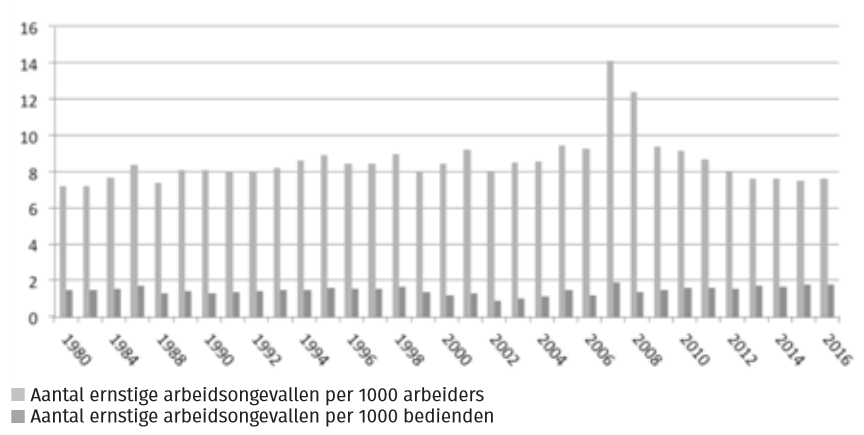
\includegraphics[width=0.7\textwidth]{arbeidsongevallen}
			\caption{Frequentiegraad ernstige arbeidsongevallen in de privésector.}
		\end{figure}
	\end{frame}

	\begin{frame}{Context}
		\begin{itemize}
			\item Mogelijke oplossing
			\begin{itemize}
				\item Het inzetten van robotica in gevaarlijke omgevingen
				\item<2-> Hoe besturen?
				\begin{itemize}
					\item Remote control
					\item Autonoom
					\item Actieherkenning
				\end{itemize}
			\end{itemize}
		\end{itemize}
	\end{frame}

	\begin{frame}\frametitle{Context}
		\begin{itemize}
			\item De verplaatsing van een robot uitvoeren met enkel actieherkenning
			\item<2-> Met de kinect sensor
			\begin{itemize}
				\item Kan skeletbeelden genereren vanuit RGB-D data
			\end{itemize}
			\begin{figure}
				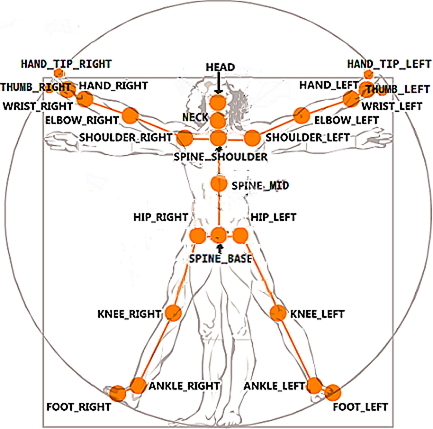
\includegraphics[width=0.4\textwidth]{skeleton}
			\end{figure}	
		\end{itemize}
	\end{frame}

	\section{Probleemstellingen}
	\begin{frame}\frametitle{Probleemstellingen}
		\begin{enumerate}
			\item Verschillen in lichaamsbouw mogelijk (klein vs groot)
			\item Verschillen in camerahoek
			\item<2-> Real-time actieherkenning
			\begin{itemize}
				\item De actie herkennen op het moment dat deze uitgevoerd wordt
			\end{itemize} 
		\end{enumerate}
		\begin{figure}
			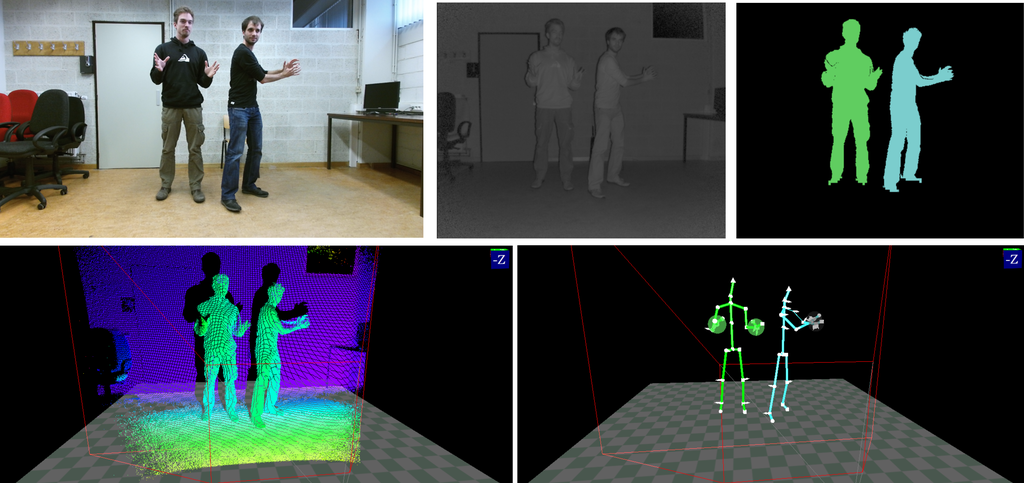
\includegraphics[width=\textwidth]{sensoren}
		\end{figure}
	\end{frame}

	\begin{frame}\frametitle{Onderzoek}
		\begin{enumerate}
			\item De features moeten rotatie- en lichaamsinvariant zijn
			\item Actie moet vroeg genoeg herkend worden om live te kunnen classificeren
		\end{enumerate}
	\end{frame}


	\section{Methodologie}
	\begin{frame}\frametitle{Methodologie}
		\begin{tikzpicture}[node distance = 2cm]
			%\node (literatuur) [process] {Literatuur};
			%\node (literatuur1) [result, right of=literatuur, xshift=2cm, yshift=0.5cm] {Features};
			%\node (literatuur2) [result, right of=literatuur, xshift=2cm, yshift=-0.5cm] {Temporale dimensie};
			\node (dataset) [process] {Dataset};
			
			\node (dataset1) [result, right of=dataset,xshift=4cm,yshift=0.5cm] {3 personen, 9 acties, elk 5 maal uitgevoerd};
			\node (dataset2) [result, right of=dataset,xshift=2cm,yshift=-0.5cm,fill=red!30] {Frame drops aanwezig};
			
			\node (experiment) [process, below of=dataset] {Experimenteerfase};
				
			\node (experiment1) [result, right of=experiment,xshift=4cm,yshift=0.5cm,fill=orange!30] {Features: HOJ3D, COV3DJ, EigenJoints};
			\node (experiment2) [result, right of=experiment,xshift=4cm,yshift=-0.5cm,fill=orange!30] {Temporale dimensie: SW, HMM, DTW};
			
			\node (evaluatie) [process, below of=experiment] {Evaluatie};
			
			%\draw [arrow] (literatuur) -- (literatuur1);
			%\draw [arrow] (literatuur) -- (literatuur2);
			%\draw [arrow] (literatuur) -- (dataset);
			\draw [arrow] (dataset) -- (dataset1);
			\draw [arrow] (dataset) -- (dataset2);
			\draw [arrow] (dataset) -- (experiment);
			\draw [arrow] (experiment) -- (experiment1);
			\draw [arrow] (experiment) -- (experiment2);
			\draw [arrow] (experiment) -- (evaluatie);
			\draw [arrow] (evaluatie) -- (experiment);
		\end{tikzpicture}
	\end{frame}
	\begin{frame}{Dataset}
		\begin{itemize}
			\item Welke acties?
			\item<2-> Frame drops
			\begin{itemize}
				\item Verouderde hardware
				\item Te hoge resolutie
			\end{itemize}
		\end{itemize}
	\end{frame}
	\begin{frame}{Experimenteerfase}
	\begin{itemize}
		\item Verschillende features uittesten op eigen dataset
		\begin{itemize}
			\item HOJ3D
			\item COV3DJ
			\item EigenJoints
		\end{itemize}
		\item Combineren met verschillende methoden om temporale informatie te behouden
		\begin{itemize}
			\item Sliding Window
			\item Dynamic Time Warping
			\item Hidden Markov Model
		\end{itemize}
		\item Zoeken naar verbeteringen
		\begin{itemize}
			\item Combinatie van features
			\item Dimensiereductie
		\end{itemize}
	\end{itemize}
	\end{frame}
	\begin{frame}{Evaluatie}
	\begin{itemize}
		\item Confusion matrix
		\begin{figure}
			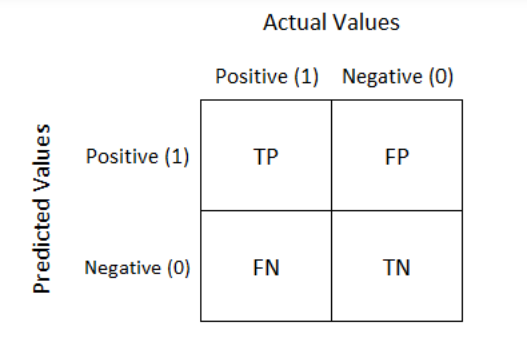
\includegraphics[width=0.5\textwidth]{confusionmatrix}
		\end{figure}
		\begin{itemize}
			\item Accuracy: $\frac{TP + TN}{TP + FP + FN + TN}$
			\item Precision: $\frac{TP}{TP + FP}$
			\item Recall: $\frac{TP}{TP + FN}$
			\item F1 score: $2\frac{P\cdot R}{P + R}$
		\end{itemize}
	\end{itemize}
	\end{frame}
	\begin{frame}
		\begin{center}
			\Huge Vragen, opmerkingen, ...?
		\end{center}
	\end{frame}
\end{document}